\chapter{Previsão de séries temporais com Regression WiSARD}
Como previsto no capítulo de redes neurais sem peso, o modelo Regression WiSARD é utilizado para resolver problemas de regressão, porém não é possível realizar previsão de séries temporais por depender de características que não são função do tempo. É possível, entretanto, tratar um problema de previsão de séries temporais como um problema de regressão aplicando técnicas como a janela deslizante e médias móveis conforme detalhado nas seções seguintes.

\section{Janelas deslizantes}
O método de janelas deslizantes é essencial para a Regression WiSARD ser capaz de realizar previsões de séries temporais. Isso ocorre porque é a técnica que permite transformar o problema temporal em um problema de regressão supervisionado.

O método consiste em tornar cada amostra dependente das $W$ amostras anteriores, e faz isso alocando uma janela de $W$ amostras no início da série temporal e deslocando até o final de amostra em amostra para formar a matriz de características, conforme ilustra a Figura~\ref{fig:sliding_window}, onde $W=3$ e $N$ é o número de registros da série temporal.

    \begin{figure}[!ht] \label{fig:sliding_window}
    \centering
    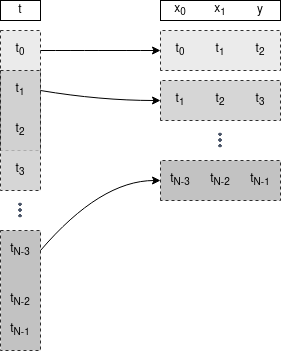
\includegraphics[width=3.0in]{img/sliding_window.png}
    \caption{Exemplo de aplicação do método de janelas deslizantes com passo $s=1$  para transformar a série temporal $t$ em uma matriz de características $X$ e um vetor alvo $y$. }
    \end{figure}

Em alguns casos, também é possível utilizar outro parâmetro para a técnica, como o tamanho do passo da janela. No exemplo da Figura~\ref{fig:sliding_window_2}, esse tamanho de passo foi considerado como $s=1$, já que o tamanho do passo para formar cada registro foi de 1.

\begin{figure}[!ht] \label{fig:sliding_window_2}
    \centering
    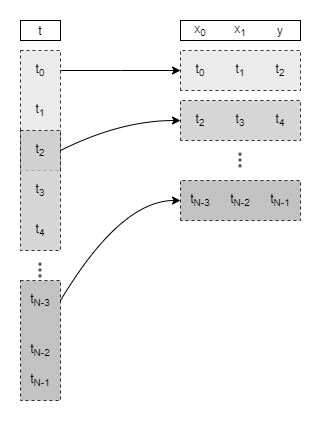
\includegraphics[width=3.0in]{img/sliding_window_2.png}
    \caption{Exemplo de aplicação do método de janelas deslizantes com passo $s=2$  para transformar a série temporal $t$ em uma matriz de características $X$ e um vetor alvo $y$. }
\end{figure}

É importante observar algumas características quanto ao método de janela deslizante, como a preservação da ordem dos registros, que é importante para garantir que a variável alvo será uma função dos dados anteriores na série temporal. Além disso, os primeiros $W$ valores da série temporal serão inutilizados, pois não possuem registros anteriores suficientes para gerar um registro na matriz de características.

A utilização deste método permite que o problema de previsão de séries temporais univariado seja resolvido como um problema de regressão supervisionado. Com os dados sendo transformados dessa forma, é possível aplicar qualquer algorítmo de regressão linear ou não linear de aprendizado de máquina.

Mesmo com a utilização desse método, os problemas relacionados à previsão de séries temporais como a flutuação de valores em um curto período. Para resolver esse tipo de problema, podem ser utilizados outros métodos, como o de médias móveis, que é explicado na Seção~\ref{sec:moving_average}.

\section{Média móvel} \label{sec:moving_average}
Existem alguns tipos de média móvel como a simples, a ponderada, a cumulativa, e a exponencial. Cada tipo de média móvel produz um efeito ao ser aplicada na série temporal, e podem ser usadas para alcançar objetivos diferentes. O algoritmo de média móvel simples, por exemplo, é utilizado para suavizar flutuações em curto prazo em uma série temporal, e consequentemente evidenciar tendências a longo prazo. Essa transformação se faz necessária, portanto, para facilitar o processo de aprendizado de modelos preditivos.

Para aplicar uma média móvel simples, dado uma sequência $P = (p_{1}, p_{2}, ..., p_{m})$ e um tamanho de janela $n$, é possível calcular cada valor $\overline{p}_{i}$ de média móvel conforme a Equação~\ref{eq:moving_average}.

\begin{equation} \label{eq:moving_average}
    \overline{p}_{i} = \dfrac{1}{n}\sum ^{i}_{j=i-n}p_{j}
\end{equation}

É possível notar que os primeiros $n$ valores da série temporal resultante são inviáveis de calcular, pois não possuem $n$ antecessores para o cáculo da média. Nesse sentido, uma abordagem simples é apenas desconsiderar os $n$ valores iniciais da série, já que em muitos casos o tamanho da série temporal é grande suficiente para essa perda não ser expressiva para os modelos preditivos.

%% Verificar na lib do pandas como é implementado e escrever a equação...

\section{Regression WiSARD}
% Explicar treinamento do modelo...

% Explicar predições com o modelo...

% Vantagens - Aprendizado em tempo real, ...
